\let\negthickspace\undefined
\documentclass[journal]{IEEEtran}
\usepackage[a5paper, margin=10mm, onecolumn]{geometry}
%\usepackage{lmodern} % Ensure lmodern is loaded for pdflatex
\usepackage{tfrupee} % Include tfrupee package
\setlength{\headheight}{1cm} % Set the height of the header box
\setlength{\headsep}{0mm}     % Set the distance between the header box and the top of the text
\usepackage{gvv-book}
\usepackage{gvv}
\usepackage{cite}
\usepackage{amsmath,amssymb,amsfonts,amsthm}
\usepackage{algorithmic}
\usepackage{graphicx}
\usepackage{textcomp}
\usepackage{xcolor}
\usepackage{txfonts}
\usepackage{listings}
\usepackage{enumitem}
\usepackage{mathtools}
\usepackage{gensymb}
\usepackage{comment}
\usepackage[breaklinks=true]{hyperref}
\usepackage{tkz-euclide} 
\usepackage{listings}
% \usepackage{gvv}                                        
\def\inputGnumericTable{}                                 
\usepackage[latin1]{inputenc}                                
\usepackage{color}                                            
\usepackage{array}                                            
\usepackage{longtable}                                       
\usepackage{calc}                                             
\usepackage{multirow}                                         
\usepackage{hhline}                                           
\usepackage{ifthen}                                           
\usepackage{lscape}
\renewcommand{\thefigure}{\theenumi}
\renewcommand{\thetable}{\theenumi}
\setlength{\intextsep}{10pt} % Space between text and floats
\numberwithin{equation}{enumi}
\numberwithin{figure}{enumi}
\renewcommand{\thetable}{\theenumi}
\begin{document}
\bibliographystyle{IEEEtran}
\title{10.3.2.7}
\author{EE24BTECH11051 - Prajwal}
% \maketitle
% \newpage
% \bigskip
{\let\newpage\relax\maketitle}
\begin{enumerate}
\item Draw the graph of the equation $x-y+1=0$ and $3x+2y-12=0$. Determine the coordinates of the vertices of the triangle formed by the lines and x-axis\\
\textbf{Solution}:-\\
Given,
\begin{align}
x-y+1=0\\
3x+2y-12=0\\
y=0
\end{align}
lines $x-y+1=0$ and $3x+2y-12=0$ touches `x-axis at,
\begin{align}
    x=-1\\
    x=4
\end{align}
Both given line touches at,
\begin{align}
    x=2\\
    y=3
\end{align}
\textbf{CODING LOGIC}\\


	Let us assume the given system of equations are consistent and we will try solving using LU decomposition
	
	Given the system of linear equations:
	\begin{align}
	x-y+1=0\\
    3x+2y-12=0\\
    y=0
	\end{align}
	
	We rewrite the equations as:
	\begin{align}
		x_1 &= x, \\
        		x_2 &= y,
	\end{align}
	giving the system:
	\begin{align}
	x_1-x_2=-1\\
    3x_1+2x_2=12\\
    x_2=0
	\end{align}
	
	\subsection*{Step 1: Convert to Matrix Form}
	We write the system as:
	\begin{align}
		A \mathbf{x} &= \mathbf{b},
	\end{align}
	where:
	\begin{align}
A_1 &= \begin{bmatrix} 1 & -1 \\ 0 & 1 \end{bmatrix},\\
A_2 &= \begin{bmatrix} 3 & 2 \\ 0 & 1 \end{bmatrix},\\
A_3 &= \begin{bmatrix} 1 & -1 \\ 3 & 2 \end{bmatrix},\\
\mathbf{x} &= \begin{bmatrix} x_1 \\ x_2 \end{bmatrix}, \\
\mathbf{b_1} &= \begin{bmatrix} -1 \\ 0 \end{bmatrix},\\
\mathbf{b_2} &= \begin{bmatrix} 12 \\ 0 \end{bmatrix},\\
\mathbf{b_3} &= \begin{bmatrix} -1 \\ 12 \end{bmatrix}.
	\end{align}
	
	\subsection*{Step 2: LU factorization using update equaitons}
    Given a matrix $ \mathbf{A} $ of size $ n \times n $, LU decomposition is performed row by row and column by column. The update equations are as follows:\\
    \textbf{Step-by-Step Procedure:}\\
1. Initialization: 
   - Start by initializing $ \mathbf{L} $ as the identity matrix $ \mathbf{L} = \mathbf{I} $ and $ \mathbf{U} $ as a copy of $ \mathbf{A} $.
   
2. Iterative Update:
   - For each pivot $ k = 1, 2, \ldots, n $:
     - Compute the entries of $ U $ using the first update equation.
     - Compute the entries of $ L $ using the second update equation.
        
3. Result:
   - After completing the iterations, the matrix $ \mathbf{A} $ is decomposed into $ \mathbf{L} \cdot \mathbf{U} $, where $ \mathbf{L} $ is a lower triangular matrix with ones on the diagonal, and $ \mathbf{U} $ is an upper triangular matrix.

    

\subsection*{1. Update for $ U_{k,j} $ (Entries of $ U $)}

For each column $ j \geq k $, the entries of $ U $ in the $ k $-th row are updated as:
\[
U_{k,j} = A_{k,j} - \sum_{m=1}^{k-1} L_{k,m} \cdot U_{m,j}, \quad \text{for } j \geq k.
\]
This equation computes the elements of the upper triangular matrix $ \mathbf{U} $ by eliminating the lower triangular portion of the matrix.

\subsection*{2. Update for $ L_{i,k} $ (Entries of $ L $)}

For each row $ i > k $, the entries of $ L $ in the $ k $-th column are updated as:
\[
L_{i,k} = \frac{1}{U_{k,k}} \left( A_{i,k} - \sum_{m=1}^{k-1} L_{i,m} \cdot U_{m,k} \right), \quad \text{for } i > k.
\]
This equation computes the elements of the lower triangular matrix $ \mathbf{L} $, where each entry in the column is determined by the values in the rows above it.\\
Using a code we get L,U as 
\begin{align}   
L_1 = \begin{bmatrix} 1 & 0 \\ 0 & 1 \end{bmatrix},
U_1 = \begin{bmatrix} 1 & -1 \\ 0 & 1 \end{bmatrix}\\
L_2 = \begin{bmatrix} 1 & 0 \\ 0 & 1 \end{bmatrix},
U_2 = \begin{bmatrix} 3 & 2 \\ 0 & 1 \end{bmatrix}\\
L_3 = \begin{bmatrix} 1 & 0 \\ 3 & 1 \end{bmatrix},
U_3 = \begin{bmatrix} 1 & -1 \\ 0 & 5 \end{bmatrix}
\end{align}

	\subsection*{Step 3: Solve $L\mathbf{y} = \mathbf{b}$ (Forward Substitution)}
	We solve:
	\begin{align}
		L_1\mathbf{y_1} = \mathbf{b_1} \quad \text{or} \quad \begin{bmatrix} 1 & 0 \\ 0 & 1 \end{bmatrix} \begin{bmatrix} y_1 \\ y_2 \end{bmatrix} = \begin{bmatrix} -1 \\ 0 \end{bmatrix}.\\
        L_2\mathbf{y_2} = \mathbf{b_2} \quad \text{or} \quad \begin{bmatrix} 1 & 0 \\ 0 & 1 \end{bmatrix} \begin{bmatrix} y_1 \\ y_2 \end{bmatrix} = \begin{bmatrix} 12 \\ 0 \end{bmatrix}.\\
        L_3\mathbf{y_3} = \mathbf{b_3} \quad \text{or} \quad \begin{bmatrix} 1 & 0 \\ 3 & 1 \end{bmatrix} \begin{bmatrix} y_1 \\ y_2 \end{bmatrix} = \begin{bmatrix} -1 \\ 15 \end{bmatrix}.
	\end{align}
	Thus:
	\begin{align}
		\mathbf{y_1} &= \begin{bmatrix} -1 \\ 0 \end{bmatrix}.\\
        \mathbf{y_2} &= \begin{bmatrix} 12 \\ 0 \end{bmatrix}.\\
        \mathbf{y_3} &= \begin{bmatrix} -12 \\ 0 \end{bmatrix}.\\
	\end{align}
    	
	\subsection*{Step 4: Solve $U\mathbf{x} = \mathbf{y}$ (Backward Substitution)}
	We solve:
	\begin{align}
		U_1\mathbf{x_1} = \mathbf{y_1} \quad \text{or} \quad \begin{bmatrix} 1 & -1 \\ 0 & 1 \end{bmatrix} \begin{bmatrix} x_1 \\ x_2 \end{bmatrix} = \begin{bmatrix} -1 \\ 0 \end{bmatrix}.\\
        U_2\mathbf{x_2} = \mathbf{y_2} \quad \text{or} \quad \begin{bmatrix} 3 & 2 \\ 0 & 1 \end{bmatrix} \begin{bmatrix} x_1 \\ x_2 \end{bmatrix} = \begin{bmatrix} 12 \\ 0 \end{bmatrix}.\\
        U_3\mathbf{x_3} = \mathbf{y_3} \quad \text{or} \quad \begin{bmatrix} 1 & -1 \\ 0 & 5 \end{bmatrix} \begin{bmatrix} x_1 \\ x_2 \end{bmatrix} = \begin{bmatrix} -12 \\ 0 \end{bmatrix}.\\
	    \mathbf{x_1} &= \begin{bmatrix} -1 \\ 0 \end{bmatrix}.\\
        \mathbf{x_2} &= \begin{bmatrix} 4 \\ 0 \end{bmatrix}.\\
        \mathbf{x_3} &= \begin{bmatrix} 2 \\ 3 \end{bmatrix}.
	\end{align}
	Hence ,there exist infinity many values of $x_1$ and $x_2$.
	So, both lines are same.
\end{enumerate}
\begin{figure}[h!]
   \centering
   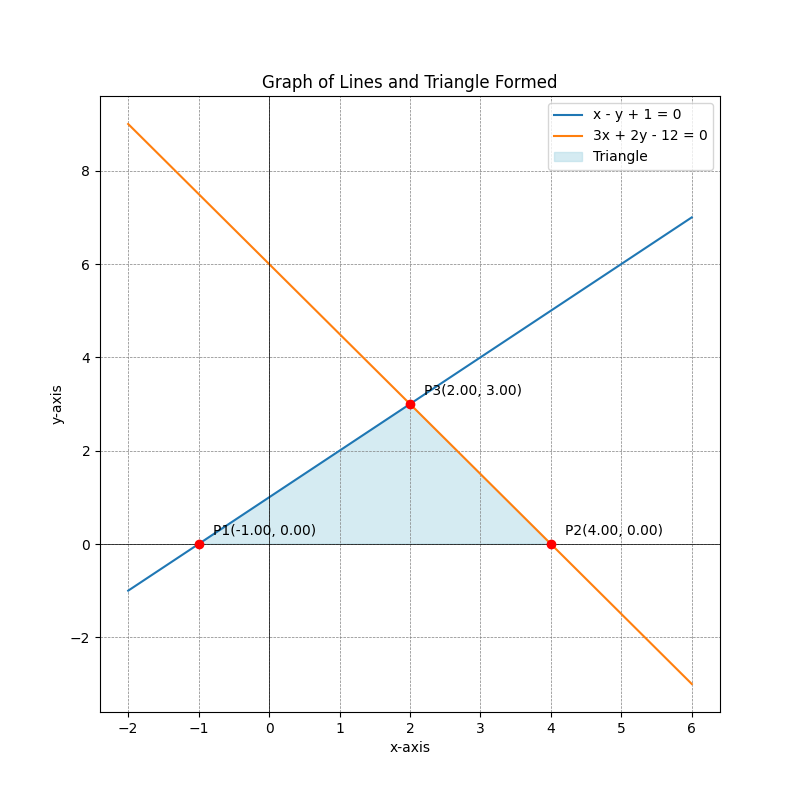
\includegraphics[width=0.7\linewidth]{figs/Figure_1.png}
\end{figure}

\end{document}
